
\documentclass[a4paper,12pt]{scrbook}
\usepackage{amsmath,amssymb,amsthm}
\usepackage{fancyvrb}
\usepackage{parskip}
\usepackage{lastpage}
\usepackage{verbatim,boxedminipage,enumitem}
\usepackage{ifthen}
\usepackage{color,graphicx}
\usepackage{pgf}
\usepackage{longtable}
\usepackage{upquote}
%\usepackage[all]{xy}
\usepackage{tobiShell}
\usepackage{tikz}
\usetikzlibrary{automata}
\usetikzlibrary{arrows}
\usepackage{pgf,pgfarrows,pgfnodes}
\usepackage{pgfplots}
\usepackage{circuitikz}
\usetikzlibrary{circuits}
\usetikzlibrary{circuits.logic.US}
\usepackage{mymath}
\usepackage{python}
%------------------------------------------------------------------
% Verbatim for console window - single line frame, no line numbers
%------------------------------------------------------------------
\DefineVerbatimEnvironment%
 {console}{Verbatim}
 {frame=single}

%--------------------------------------------------------
% Remove the vertical spacing before and after Verbatim.
%--------------------------------------------------------
\usepackage{atbeginend}
\BeforeBegin{console}{\mbox{}\\ \begin{minipage}{\textwidth}\vspace{3pt}}
\AfterEnd{console}{\vspace{4pt} \end{minipage} \\ }

\begin{document}
\thispagestyle{empty}

\begin{center}
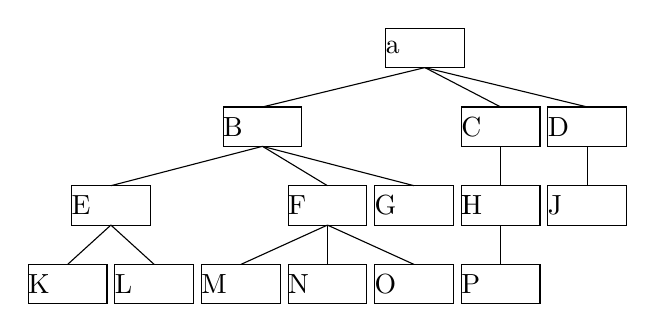
\begin{tikzpicture}

\draw (4.5375, 0.0)
  node[draw, , , color=black,
       rounded corners=0.0cm, inner sep=0.0cm] {

\begin{minipage}[c][0.5cm]{1.0cm}
\mbox{}

\end{minipage}

};
\draw (4.5375, 0.0) node[color=black,
 inner sep=0.0cm] {
 
\begin{minipage}[c][0.5cm]{1.0cm}
a
\end{minipage}

};
\draw (5.5, -1.0)
  node[draw, , , color=black,
       rounded corners=0.0cm, inner sep=0.0cm] {

\begin{minipage}[c][0.5cm]{1.0cm}
\mbox{}

\end{minipage}

};
\draw (5.5, -1.0) node[color=black,
 inner sep=0.0cm] {
 
\begin{minipage}[c][0.5cm]{1.0cm}
C
\end{minipage}

};
\draw (2.475, -1.0)
  node[draw, , , color=black,
       rounded corners=0.0cm, inner sep=0.0cm] {

\begin{minipage}[c][0.5cm]{1.0cm}
\mbox{}

\end{minipage}

};
\draw (2.475, -1.0) node[color=black,
 inner sep=0.0cm] {
 
\begin{minipage}[c][0.5cm]{1.0cm}
B
\end{minipage}

};
\draw (0.55, -2.0)
  node[draw, , , color=black,
       rounded corners=0.0cm, inner sep=0.0cm] {

\begin{minipage}[c][0.5cm]{1.0cm}
\mbox{}

\end{minipage}

};
\draw (0.55, -2.0) node[color=black,
 inner sep=0.0cm] {
 
\begin{minipage}[c][0.5cm]{1.0cm}
E
\end{minipage}

};
\draw (6.6, -1.0)
  node[draw, , , color=black,
       rounded corners=0.0cm, inner sep=0.0cm] {

\begin{minipage}[c][0.5cm]{1.0cm}
\mbox{}

\end{minipage}

};
\draw (6.6, -1.0) node[color=black,
 inner sep=0.0cm] {
 
\begin{minipage}[c][0.5cm]{1.0cm}
D
\end{minipage}

};
\draw (4.4, -2.0)
  node[draw, , , color=black,
       rounded corners=0.0cm, inner sep=0.0cm] {

\begin{minipage}[c][0.5cm]{1.0cm}
\mbox{}

\end{minipage}

};
\draw (4.4, -2.0) node[color=black,
 inner sep=0.0cm] {
 
\begin{minipage}[c][0.5cm]{1.0cm}
G
\end{minipage}

};
\draw (3.3, -2.0)
  node[draw, , , color=black,
       rounded corners=0.0cm, inner sep=0.0cm] {

\begin{minipage}[c][0.5cm]{1.0cm}
\mbox{}

\end{minipage}

};
\draw (3.3, -2.0) node[color=black,
 inner sep=0.0cm] {
 
\begin{minipage}[c][0.5cm]{1.0cm}
F
\end{minipage}

};
\draw (5.5, -2.0)
  node[draw, , , color=black,
       rounded corners=0.0cm, inner sep=0.0cm] {

\begin{minipage}[c][0.5cm]{1.0cm}
\mbox{}

\end{minipage}

};
\draw (5.5, -2.0) node[color=black,
 inner sep=0.0cm] {
 
\begin{minipage}[c][0.5cm]{1.0cm}
I
\end{minipage}

};
\draw (5.5, -2.0)
  node[draw, , , color=black,
       rounded corners=0.0cm, inner sep=0.0cm] {

\begin{minipage}[c][0.5cm]{1.0cm}
\mbox{}

\end{minipage}

};
\draw (5.5, -2.0) node[color=black,
 inner sep=0.0cm] {
 
\begin{minipage}[c][0.5cm]{1.0cm}
H
\end{minipage}

};
\draw (0.0, -3.0)
  node[draw, , , color=black,
       rounded corners=0.0cm, inner sep=0.0cm] {

\begin{minipage}[c][0.5cm]{1.0cm}
\mbox{}

\end{minipage}

};
\draw (0.0, -3.0) node[color=black,
 inner sep=0.0cm] {
 
\begin{minipage}[c][0.5cm]{1.0cm}
K
\end{minipage}

};
\draw (6.6, -2.0)
  node[draw, , , color=black,
       rounded corners=0.0cm, inner sep=0.0cm] {

\begin{minipage}[c][0.5cm]{1.0cm}
\mbox{}

\end{minipage}

};
\draw (6.6, -2.0) node[color=black,
 inner sep=0.0cm] {
 
\begin{minipage}[c][0.5cm]{1.0cm}
J
\end{minipage}

};
\draw (2.2, -3.0)
  node[draw, , , color=black,
       rounded corners=0.0cm, inner sep=0.0cm] {

\begin{minipage}[c][0.5cm]{1.0cm}
\mbox{}

\end{minipage}

};
\draw (2.2, -3.0) node[color=black,
 inner sep=0.0cm] {
 
\begin{minipage}[c][0.5cm]{1.0cm}
M
\end{minipage}

};
\draw (1.1, -3.0)
  node[draw, , , color=black,
       rounded corners=0.0cm, inner sep=0.0cm] {

\begin{minipage}[c][0.5cm]{1.0cm}
\mbox{}

\end{minipage}

};
\draw (1.1, -3.0) node[color=black,
 inner sep=0.0cm] {
 
\begin{minipage}[c][0.5cm]{1.0cm}
L
\end{minipage}

};
\draw (4.4, -3.0)
  node[draw, , , color=black,
       rounded corners=0.0cm, inner sep=0.0cm] {

\begin{minipage}[c][0.5cm]{1.0cm}
\mbox{}

\end{minipage}

};
\draw (4.4, -3.0) node[color=black,
 inner sep=0.0cm] {
 
\begin{minipage}[c][0.5cm]{1.0cm}
O
\end{minipage}

};
\draw (3.3, -3.0)
  node[draw, , , color=black,
       rounded corners=0.0cm, inner sep=0.0cm] {

\begin{minipage}[c][0.5cm]{1.0cm}
\mbox{}

\end{minipage}

};
\draw (3.3, -3.0) node[color=black,
 inner sep=0.0cm] {
 
\begin{minipage}[c][0.5cm]{1.0cm}
N
\end{minipage}

};
\draw (5.5, -3.0)
  node[draw, , , color=black,
       rounded corners=0.0cm, inner sep=0.0cm] {

\begin{minipage}[c][0.5cm]{1.0cm}
\mbox{}

\end{minipage}

};
\draw (5.5, -3.0) node[color=black,
 inner sep=0.0cm] {
 
\begin{minipage}[c][0.5cm]{1.0cm}
P
\end{minipage}

};\draw[black] (4.5375,-0.25) -- (2.475,-0.75);
\draw[black] (4.5375,-0.25) -- (5.5,-0.75);
\draw[black] (4.5375,-0.25) -- (6.6,-0.75);
\draw[black] (5.5,-1.25) -- (5.5,-1.75);
\draw[black] (5.5,-1.25) -- (5.5,-1.75);
\draw[black] (2.475,-1.25) -- (0.55,-1.75);
\draw[black] (2.475,-1.25) -- (3.3,-1.75);
\draw[black] (2.475,-1.25) -- (4.4,-1.75);
\draw[black] (0.55,-2.25) -- (0.0,-2.75);
\draw[black] (0.55,-2.25) -- (1.1,-2.75);
\draw[black] (6.6,-1.25) -- (6.6,-1.75);
\draw[black] (3.3,-2.25) -- (2.2,-2.75);
\draw[black] (3.3,-2.25) -- (3.3,-2.75);
\draw[black] (3.3,-2.25) -- (4.4,-2.75);
\draw[black] (5.5,-2.25) -- (5.5,-2.75);
\end{tikzpicture}

\end{center}

\end{document}
